\whiteBGstarBegin

\begin{enumerate}[label=\bfseries Câu \arabic*:]
	
	\item \mkstar{1}
	
	\cauhoi
	{Định luật I Niu-tơn xác nhận rằng
		\begin{mcq}
			\item do quán tính nên mọi vật đang chuyển động đều có xu hướng dừng lại.
			\item với mỗi lực tác dụng đều có một phản lực trực đối.
			\item vật giữ nguyên trạng thái đứng yên hoặc chuyển động thẳng đều khi nó không chịu tác dụng của bất kì lực nào.
			\item khi hợp lực tác dụng lên vật bằng 0 thì vật không thể chuyển động được.
		\end{mcq}
	}
	
	\loigiai
	{\textbf{Đáp án: C.}
		
		Định luật I - Niu-tơn: Nếu một vật không chịu tác dụng của lực nào hoặc chịu tác dụng của các lực có hợp lực bằng không, thì nó giữ nguyên trạng thái đứng yên hoặc chuyển động thẳng đều.
		
		
	}
	\item \mkstar{1}
	
	\cauhoi
	{Hai lực trực đối cân bằng là hai lực
		\begin{mcq}
			\item tác dụng vào cùng một vật.
			\item không bằng nhau về độ lớn.
			\item bằng nhau về độ lớn nhưng không nhất thiết phải cùng giá.
			\item có cùng độ lớn, cùng phương, ngược chiều, tác dụng vào hai vật khác nhau.
		\end{mcq}
	}
	\loigiai
	{\textbf{Đáp án: D.}
		
		Hai lực trực đối cân bằng là hai lực có cùng độ lớn, cùng phương, ngược chiều, tác dụng vào hai vật khác nhau.
		
		
	}
	\item \mkstar{1}
	
	\cauhoi
	{Kết luận nào sau đây đúng?
		\begin{mcq}
			\item Nếu không có lực tác dụng vào vật thì vật không thể chuyển động được.
			\item Không cần có lực tác dụng vào vật thì vật vẫn có thể chuyển động tròn đều được.
			\item Lực là nguyên nhân duy trì chuyển động của một vật.
			\item Lực là nguyên nhân làm biến đổi chuyển động của một vật.
		\end{mcq}
	}
	
	\loigiai
	{\textbf{Đáp án: D.}
		
		Lực là nguyên nhân làm biến đổi chuyển động của một vật.
		
		
	}
	\item \mkstar{2}
	
	\cauhoi
	{Trường hợp nào sau đây có liên quan đến quán tính?
		\begin{mcq}(2)
			\item Vật rơi tự do.
			\item Vật rơi trong không khí.
			\item Chiếc bè trôi trên sông.
			\item Giũ quần áo cho sạch bụi.
		\end{mcq}
	}
	
	\loigiai
	{\textbf{Đáp án: D.}	
		
		Quán tính là tính chất của mọi vật có xu hướng bảo toàn vận tốc cả về hướng và độ lớn.
		
		
	}
	\item \mkstar{2}
	
	\cauhoi
	{Vật nào sau đây chuyển động theo quán tính?
		\begin{mcq}
			\item Vật chuyển động tròn đều.
			\item Vật chuyển động trên quỹ đạo thẳng.
			\item Vật chuyển động thẳng đều.
			\item Vật chuyển động khi tất cả các lực tác dụng lên vật mất đi.
		\end{mcq}
	}
	
	\loigiai
	{\textbf{Đáp án: D.}
		
	Chuyển động theo quán tính là chuyển động khi tất cả các lực tác dụng lên vật mất đi.
		
		
	}
	\item \mkstar{2}
	
	\cauhoi
	{Người ta dùng búa đóng một cây đinh vào một khối gỗ.
		\begin{mcq}
			\item Lực do đinh tác dụng vào búa lớn hơn lực do búa tác dụng vào đinh.
			\item Lực do đinh tác dụng vào búa nhỏ hơn lực do búa tác dụng vào đinh.
			\item Lực do đinh tác dụng vào búa bằng lực do búa tác dụng vào đinh.
			\item Lực do đinh tác dụng vào búa có thể lớn hơn hoặc nhỏ hơn lực do búa tác dụng vào đinh.
		\end{mcq}
	}
	
	\loigiai
	{\textbf{Đáp án: C.}
		
		Cặp lực trực đối trong định luật III Niu-tơn bằng nhau về độ lớn.
		
		
	}
	\item \mkstar{2}
	
	\cauhoi
	{Các lực tác dụng vào vật cân bằng nhau khi vật
		\begin{mcq}(2)
			\item chuyển động thẳng đều.
			\item chuyển động thẳng biến đổi đều.
			\item chuyển động thẳng.
			\item chuyện động tròn đều
		\end{mcq}
	}
	
	\loigiai
	{\textbf{Đáp án: A.}
		
		Các lực tác dụng vào vật cân bằng nhau khi vật chuyển động không có gia tốc ($\vec a = 0$), bao gồm chuyển động thẳng đều.
		
		
	}
	\item \mkstar{2}
	
	\cauhoi
	{Một vật đang chuyển động với vận tốc $3\ \text{m/s}$. Nếu bỗng nhiên các lực tác dụng lên nó mất đi thì
		\begin{mcq}
			\item vật dừng lại ngay.
			\item vật đổi hướng chuyển động.
			\item vật chuyển động chậm dần rồi mới dừng lại.
			\item vật tiếp tục chuyển động như cũ.
		\end{mcq}
	}
	
	\loigiai
	{\textbf{Đáp án: D.}
		
		Định luật I - Niu-tơn: Nếu một vật không chịu tác dụng của lực nào hoặc chịu tác dụng của các lực có hợp lực bằng không, thì nó giữ nguyên trạng thái đứng yên hoặc chuyển động thẳng đều.
		
		
	}
	\item \mkstar{2}
	
	\cauhoi
	{Kết luận nào sau đây đúng?
		\begin{mcq}
			\item Khi vật không chịu tác dụng của lực nào thì vật phải đứng yên.
			\item Một vật có thể chịu tác dụng đồng thời của nhiều lực mà vẫn đứng yên.
			\item Một vật không thể chuyển động được nếu không có lực nào tác dụng vào nó.
			\item Các vật luôn chuyển động theo phương của lực tác dung.
		\end{mcq}
	}
	
	\loigiai
	{\textbf{Đáp án: B.}
		
		Một vật có thể chịu tác dụng của đồng thời nhiều lực (cân bằng) mà vẫn đứng yên. Một vật không chịu tác dụng của lực nào thì vẫn có thể chuyển động thẳng đều theo quán tính.
		
		
	}
	\item \mkstar{2}
	
	\cauhoi
	{Hai xe A ($m_\text A$) và xe B ($m_\text B$) đang chuyển động với cùng một vận tốc thì tắt máy và chịu cùng lực tác dụng của một lực hãm $F$ như nhau. Sau khi chịu lực hãm, xe A còn đi thêm một đoạn $s_\text A$, xe B còn đi thêm một đoạn $s_\text B$ nữa cho đến khi dừng hẳn. Biết $s_\text B < s_\text A$, điều nào sau đây là đúng khi so sánh khối lượng của hai xe?
		\begin{mcq}(2)
			\item $m_\text A > m_\text B$.
			\item $m_\text A < m_\text B$.
			\item $m_\text A = m_\text B$
			\item Chưa đủ điều kiện để kết luận.
		\end{mcq}
	}
	
	\loigiai
	{\textbf{Đáp án: A.}
		
		Khối lượng đặc trưng cho mức quán tính của một vật, vật có khối lượng lớn hơn thì có xu hướng giữ nguyên vận tốc lớn hơn. Vậy khi $s_\text B < s_\text A$ thì $m_\text A > m_\text B$.
		
		
	}
	\item \mkstar{2}
	
	\cauhoi
	{Trong trường hợp nào dưới đây, vật chuyển động theo hướng của hợp lực tác dụng vào vật?
		\begin{mcq}
			\item Vật chuyển động thẳng đều.
			\item Vật chuyển động thẳng nhanh dần đều.
			\item Vật chuyển động thẳng chậm dần đều.
			\item Vật chuyển động tròn đều.
		\end{mcq}
	}
	
	\loigiai
	{\textbf{Đáp án: B.}
		
		Khi vật chuyển động thẳng nhanh dần đều thì $\vec a$ cùng phương, cùng chiều với $\vec v$. Do đó $\vec v$ cùng phương, cùng chiều với $\vec F$.
		
		
	}
	\item \mkstar{3}
	
	\cauhoi
	{Một lực có độ lớn $\SI{2}{\newton}$ tác dụng vào một vật có khối lượng $\SI{1}{\kilogram}$ lúc đầu đứng yên. Quãng đường mà vật đi được trong khoảng thời gian $\SI{2}{\second}$ là
		\begin{mcq}(4)
			\item $\SI{4}{\meter}$.
			\item $\SI{1}{\meter}$.
			\item $\SI{0,5}{\meter}$.
			\item $\SI{2}{\meter}$.
		\end{mcq}
	}
	
	\loigiai
	{\textbf{Đáp án: A.}
		
		Áp dụng công thức $a=\dfrac{F}{m}$ và $s=v_0t+\dfrac{at^2}{2}$.
		
		Suy ra $s=\SI{4}{\meter}$.
		
		
	}
	\item \mkstar{3}
	
	\cauhoi
	{Một vật đang đứng yên, được truyền một lực $F$ thì vận tốc tăng thêm $\SI{2}{\meter / \second}$ sau $\SI{5}{\second}$. Nếu giữ nguyên hướng của lực mà tăng độ lớn lên gấp 2 thì vận tốc của vật sau $\SI{8}{\second}$ sẽ tăng thêm bao nhiêu?
		\begin{mcq}(4)
			\item $\SI{4}{\meter / \second}$.
			\item $\SI{6.4}{\meter / \second}$.
			\item $\SI{3.2}{\meter / \second}$.
			\item $\SI{2}{\meter / \second}$.
		\end{mcq}
	}
	
	\loigiai
	{\textbf{Đáp án: B.}
		
		Gia tốc của vật dưới tác dụng của lực $F$: $a=\dfrac{\Delta v}{\Delta t}=\SI{0.4}{\meter / \second \squared}$.
		
		Gia tốc của vật dưới tác dụng của lực $2F$: $a'=\dfrac{2F}{m}=2a=\SI{0.8}{\meter / \second \squared}$.
		
		Vận tốc của vật sau tăng thêm sau $\SI{8}{\second}$: $\Delta v= a' \Delta t'=\SI{6.4}{\meter / \second}$.
		
		
	}
	\item \mkstar{3}
	
	\cauhoi
	{Một quả bóng khối lượng $\SI{200}{\gram}$ bay với vận tốc $\SI{90}{\kilo\meter/\hour}$ đến đập vuông góc vào tường rồi bật trở lại theo phương cũ với vận tốc $\SI{54}{\kilo\meter/\hour}$. Thời gian va chạm giữa bóng và tường là $\SI{0,05}{\second}$. Độ lớn lực của tường tác dụng lên quả bóng là
		\begin{mcq}(4)
			\item $\SI{160}{\newton}$.
			\item $\SI{200}{\newton}$.
			\item $\SI{210}{\newton}$.
			\item $\SI{120}{\newton}$.
		\end{mcq}
	}
	
	\loigiai
	{\textbf{Đáp án: A.}
		
		Chọn chiều dương cùng chiều bật ra của quả bóng.
		
		Áp dụng định luật II và III Newton:
		$$F_\text{tường}=F_\text{bóng}=ma=m\dfrac {v-v_0}{\Delta t}=\SI{0,2}{\kilogram}\cdot\dfrac{\SI{15}{\meter/\second}-(\SI{-25}{\meter/\second})}{\SI{0,05}{\second}}=\SI{160}{\newton}.$$
		
		
	}
	\item \mkstar{3}
	
	\cauhoi
	{Một ô tô có khối lượng 1 tấn đang chuyển động với $v=54\ \text{km/h}$ thì tắt máy, hãm phanh, chuyển động chậm dần đều. Biết độ lớn lực hãm $3000\ \text N$. Xác định quãng đường xe đi được cho đến khi dừng lại.
		\begin{mcq}(4)
			\item $32,5\ \text m$.
			\item $37,5\ \text m$.
			\item $42,5\ \text m$.
			\item $47,5\ \text m$.
		\end{mcq}
	}
	
	\loigiai
	{\textbf{Đáp án: B.}
		
		Chọn chiều dương là chiều chuyển động, gốc thời gian lúc bắt đầu hãm phanh.
		
		Áp dụng định luật II Newton:
		\[ \vec a = \dfrac {\vec F}{m} \Rightarrow a=\dfrac{F}{m} = \dfrac{-3000}{1000} = -3\ \text{m/s}^2\]
		
		Mà $v^2 - v_0 ^2 = 2as$, suy ra $s=37,5\ \text m$.
		
		
	}
	\item \mkstar{3}
	
	\cauhoi
	{Một người đang đi xe đạp với vận tốc $V_0$ thì ngừng đạp và hãm phanh. Xe đi tiếp được $40\ \text m$ thì dừng lại. Lực hãm và lực ma sát có tổng độ lớn $14\ \text N$. Khối lượng cả người và xe là $70\ \text {kg}$. Tính $V_0$.
		\begin{mcq}(4)
			\item $V_0 = 2\ \text{m/s}$.
			\item $V_0= 3\ \text{m/s}$.
			\item $V_0= 4\ \text{m/s}$.
			\item $V_0=5\ \text{m/s}$.
		\end{mcq}
	}
	
	\loigiai
	{\textbf{Đáp án: C.}	
		
		Gia tốc của xe:
		\[a=\dfrac{F}{m}=\dfrac{-14}{70} = -0,2\ \text{m/s}^2\]
		
		Mà $0-V_0^2 = 2as \Rightarrow V_0 = 4\ \text{m/s}$
		
		
	}
	\item \mkstar{3}
	
	\cauhoi
	{Một xe tải khối lượng 1 tấn, sau khi khởi hành được $10\ \text s$ đạt vận tốc $18\ \text{km/h}$. Biết lực cản mà mặt đường tác dụng lên xe là $500\ \text N$. Tính lực phát động của động cơ.
		\begin{mcq}(4)
			\item $500\ \text N$.
			\item $750\ \text N$.
			\item $1000\ \text N$.
			\item $1500\ \text N$.
		\end{mcq}
	}
	
	\loigiai
	{\textbf{Đáp án: C.}
		
		Gia tốc của xe:
		\[a = \dfrac{v-v_0}{\Delta t} = \dfrac{1}{2}\ \text{m/s}^2\]
		
		Mà $F-F_\text c = ma \Rightarrow F = F_\text c + ma = 500 + 500 = 1000\ \text N$
		
		
	}
	\item \mkstar{4}
	
	\cauhoi
	{Một viên bi A có khối lượng $\SI{300}{\gram}$ đang chuyển động với vận tốc $\SI{3}{\meter / \second}$ thì va chạm vào viên bi B có khối lượng $\SI{600}{\gram}$ đang đứng yên trên mặt bàn nhẵn nằm ngang. Biết thời gian diễn ra va chạm là $\SI{0.2}{\second}$. Sau va chạm, viên bi B chuyển động với vận tốc $\SI{0.5}{\meter}$ cùng chiều chuyển động ban đầu của bi A. Tốc độ chuyển động của bi A sau va chạm là
		\begin{mcq}(4)
			\item $\SI{1}{\meter / \second}$.
			\item $\SI{3}{\meter / \second}$.
			\item $\SI{4}{\meter / \second}$.
			\item $\SI{2}{\meter / \second}$.
		\end{mcq}
	}
	
	\loigiai
	{\textbf{Đáp án: C.}
		
		Ta xét chuyển động của viên bi B: Trước va chạm có vận tốc $v_\text B = \SI{0}{\meter / \second}$, sau va chạm có vận tốc $v_\text B'=\SI{0.5}{\meter/ \second}$. Suy ra $a_\text B=\dfrac{v_\text B'-v_\text B}{\Delta t}=\SI{2.5}{\meter / \second \squared}$.
		
		Áp dụng định luật II và III Niu-tơn:
		$|F_\text {AB}| = |F_\text {BA}| \Leftrightarrow m_\text A a_\text A = m_\text B a_\text B \Rightarrow a_\text A = \SI{5}{\meter / \second \squared}$.
		
		Vận tốc của bi A sau va chạm: $a_\text A = \dfrac{v_\text A'-v_\text A}{\Delta t}\Rightarrow v_\text A' = \SI{4}{\meter / \second}$.
		
		
	}
	\item \mkstar{4}
	
	\cauhoi
	{Cho cơ hệ như hình vẽ. Vật A có khối lượng $m_1=200\ \text g$, vật B có khối lượng $m_2=120\ \text g$ nối với nhau bởi một sợi dây nhẹ, không dãn. Hệ số ma sát trượt giữa hai vật và mặt phẳng ngang là $\mu = 0,4$. Tác dụng vào A một lực kéo $\vec F$ theo phương ngang. Biết rằng dây nối hai vật chỉ chịu được lực căng tối đa $T_0=0,6\ \text N$. Lấy $g=10\ \text{m/s}^2$. Tìm lực $F$ lớn nhất để dây không bị đứt.
		\begin{center}
			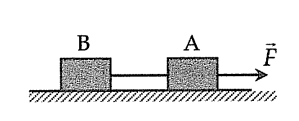
\includegraphics[scale=0.8]{../figs/VN11-Y21-PH-SYL-007-1}
		\end{center}
		\begin{mcq}(4)
			\item $0,96\ \text N$.
			\item $0,375\ \text N$.
			\item $1,5\ \text N$.
			\item $1,6\ \text N$.
		\end{mcq}
	}
	
	\loigiai
	{\textbf{Đáp án: D.}
		
		\begin{center}
			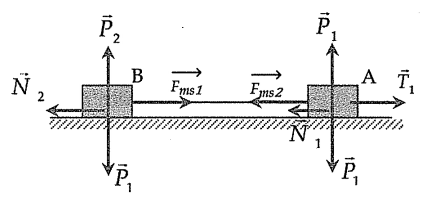
\includegraphics[scale=0.8]{../figs/VN11-Y21-PH-SYL-007-2}
		\end{center}
		
		Áp dụng định luật II Niu-tơn cho hệ vật:
		\[F-\mu (m_1 + m_2)g=(m_1+m_2)a \Rightarrow a = \dfrac{F}{m_1 + m_2} - \mu g\]
		
		Áp dụng định luật II Niu-tơn cho vật B:
		\[T-\mu m_2g=m_2 a \Rightarrow T = (\mu g + a)m_2 = \dfrac{F m_2}{m_1 + m_2} \Rightarrow F = \dfrac{m_1 + m_2}{m_2}T\]
		
		Do dây chỉ chịu được lực căng tối đa $0,6\ \text N$, nên thay số ta tính được $F$ tối đa là $F=1,6\ \text N$.
		
		
	}
	\item \mkstar{4}
	
	\cauhoi
	{Cho cơ hệ như hình vẽ. Mặt phẳng nghiêng cố định, nghiêng góc $\alpha$ so với phương ngang. Hai chất điểm khối lượng $m_1$, $m_2$ được nối với nhau bởi dây nhẹ, không dãn vắt qua ròng rọc nhẹ có kích thước không đáng kể. Biết rằng $m_2 > m_1 \sin \alpha$. Bỏ qua mọi ma sát, cho gia tốc trọng trường là $g$. Thả hai vật chuyển động tự do, tìm gia tốc của mỗi vật.
		\begin{center}
			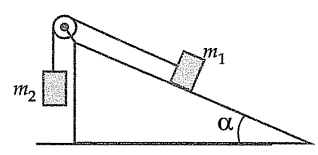
\includegraphics[scale=0.8]{../figs/VN11-Y21-PH-SYL-007-3}
		\end{center}
		
		\begin{mcq}(2)
			\item $a_1=a_2 = \dfrac{m_2 - m_1 \sin \alpha}{m_1 + m_2}g$.
			\item $a_1=a_2 = \dfrac{m_2 - m_1 \sin \alpha}{m_1 - m_2}g$.
			\item $a_1=a_2 = \dfrac{m_2 + m_1 \sin \alpha}{m_1 + m_2}g$.
			\item $a_1=a_2 = \dfrac{(m_2 - m_1) \sin \alpha}{m_1 + m_2}g$.
		\end{mcq}
	}
	
	\loigiai
	{\textbf{Đáp án: A.}
		
		\begin{center}
			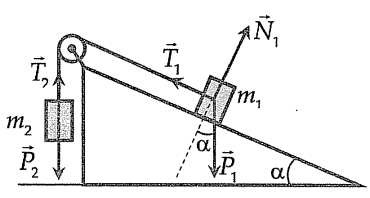
\includegraphics[scale=0.8]{../figs/VN11-Y21-PH-SYL-007-4}
		\end{center}
		
		Do $m_2 > m_1 \sin \alpha$ nên $m_2$ sẽ đi xuống.
		
		Áp dụng định luật II Niu-tơn cho mỗi vật:
		\begin{align*}
			\vec T_1 + \vec N + \vec P_1 &= m_1 \vec a_1 \\
			\vec T_2 + \vec P_2 &= m_2 \vec a_2
		\end{align*}
		
		Do dây nhẹ, không dãn, ròng rọc không khối lượng nên $T_1 = T_2 = T$, $a_1 = a_2 = a$.
		
		Chiếu các vectơ lên phương chuyển động của mỗi vật, ta được:
		\begin{align*}
			T - P_1 \sin \alpha &= m_1 a \\
			-T + P_2 &= m_2 a
		\end{align*}
		
		Suy ra $a=\dfrac{m_2 - m_1 \sin \alpha}{m_1 + m_2}g$.
		
		
	}
\end{enumerate}

\whiteBGstarEnd

\loigiai{\begin{center}
		\textbf{BẢNG ĐÁP ÁN}
	\end{center}
	\begin{center}
		\begin{tabular}{|m{2.8em}|m{2.8em}|m{2.8em}|m{2.8em}|m{2.8em}|m{2.8em}|m{2.8em}|m{2.8em}|m{2.8em}|m{2.8em}|}
			\hline
			1. C & 2. D & 3. D & 4. D & 5. D & 6. C & 7. A & 8. D & 9. B & 10. A \\
			\hline
			11. B & 12. A & 13. B & 14. A & 15. B & 16. C & 17. C & 18. C & 19. D & 20. A \\
			\hline
			
		\end{tabular}
\end{center}}